\documentclass[a4]{beamer}
\usepackage{amssymb}
\usepackage{graphicx}
\usepackage{subfigure}
\usepackage{newlfont}
\usepackage{amsmath,amsthm,amsfonts}
%\usepackage{beamerthemesplit}
\usepackage{pgf,pgfarrows,pgfnodes,pgfautomata,pgfheaps,pgfshade}
\usepackage{mathptmx}  % Font Family
\usepackage{helvet}   % Font Family
\usepackage{color}


\setbeamercovered{dynamic}

\title[MA4704]{Technology Mathematics 4 (Statistics) \\ {\normalsize MA4704 Lecture 4A}}
\author[Kevin O'Brien]{Kevin O'Brien \\ {\scriptsize Kevin.obrien@ul.ie}}
\date{Spring Semester 2013}
\institute[Maths \& Stats]{Dept. of Mathematics \& Statistics, \\ University \textit{of} Limerick}

\renewcommand{\arraystretch}{1.5}

\begin{document}

\begin{frame}
\titlepage
\end{frame}
%---------------------------------------------------------------------%
\frame{
\frametitle{Binomial Expected Value and Variance}
\begin{itemize}
\item Lecture is called off for Thursday of Week 4.
\item The first midterm is to take place Thursday of Week 5.
\item The first midterm will cover:
\begin{itemize}
\item Basic Probability
\item Descriptive statistics (mean, median variance etc)
\item Discrete probability distributions (binomial and Poisson)
\item The exponential distribution
\item (The normal distribution will be not be included).
\end{itemize}
\end{itemize}
}
%------------------------------------------------------------------%
\frame{
\frametitle{Binomial Expected Value and Variance}


If the random variable X has a binomial distribution with parameters n
and p, we write
\[ X \sim B(n,p) \]

Expectation and Variance
If $X \sim B(n,p)$, then:

\begin{itemize}
\item Expected Value of X : E(X) = np
\item Variance of X : Var(X) = np(1-p)
\end{itemize}
}
%---------------------------------------------------------------------%
\begin{frame}
\frametitle{Binomial Distribution: Example 1}
\begin{itemize} \item Diagrams of the probability mass functions of the two binomial
distributions $B(10, 0.5)$ and $B(10, 0.25)$ are shown in the bar-plots (next slide). \item Which
is which? Give a reason for your answer.
\end{itemize}
\end{frame}
%---------------------------------------------------------------------%
\begin{frame}
\frametitle{Binomial Distribution}
\begin{figure}
  % Requires \usepackage{graphicx}
  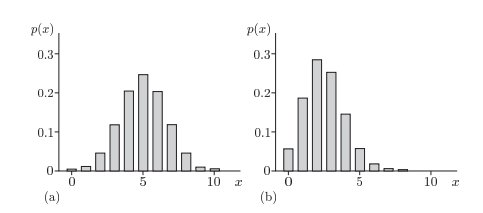
\includegraphics[scale=0.60]{4ABarCharts.jpg}\\
  \caption{Bar Charts}
\end{figure}
\end{frame}
%---------------------------------------------------------------------%
\begin{frame}
\frametitle{Binomial Distribution: Example 1}
\begin{itemize}
\item Figure A is $B(10, 0.5)$ and Figure B is $B(10, 0.25)$.
\item The mean of B(10, 0.5) is 5, and the mean of B(10, 0.25) is 2.5.
\item Also the variance of a binomial distribution corresponding to $B(10, 0.25)$ is $1.875$ ,while for $B(10, 0.25)$ it is $2.500$.
\item A visual inspection of the two bar-charts indicates that Figure A has the higher variance.
\end{itemize}
\end{frame}
%---------------------------------------------------------------------%
\begin{frame}
\frametitle{Binomial Distribution: Example 2}

\begin{itemize}
\item Components are placed into containers containing 100 items.
\item After an inspection of a large number of containers the average number of defective items was found to be 10 with a standard deviation of three.
\item Is the binomial distribution a good useful distribution, given the observed data?
\end{itemize}
\end{frame}
%---------------------------------------------------------------------%
\begin{frame}
\frametitle{Binomial Distribution: Example 2}

\begin{itemize}
\item Let the number of containers be the number of independent trials is $n=100$.
\item A success may be defined as a defective component.
\item The probability of a success is approximate $p=0.10$. (The probability of ``failure" is $1-p=0.9$).
\item The expected number of defective components is $np=10$, which concurs with our observed data.
\item The variance is computed as \[np(1-p) = 100 \times 0.1 \times 0.9 = 9\]
\item The observed standard deviation is 3 units, i.e. a variance of 9 square units.
\item Yes the binomial distribution is useful in this case.
\end{itemize}
\end{frame}
%------------------------------------------------------------------%
\frame{
\frametitle{Poisson Expected Value and Variance}


If the random variable X has a Poisson distribution with parameter $m$, we write
\[ X \sim Poisson(m) \]


\begin{itemize}
\item Expected Value of X : E(X) = m
\item Variance of X : $Var(X) = m$
\item Standard Deviation of X : $SD(X) = \sqrt{m}$
\end{itemize}
}
%------------------------------------------------------------------%
\frame{
\frametitle{Poisson Distribution : Example} 

\begin{itemize}
\item The number of faults in a fibre optic cable were recorded for each kilometre length of cable.
\item The mean number of faults was found to be 4 faults per kilometre.
\item The standard deviation of the number of faults was found to be 2 faults per kilometre.
\item Is the Poisson Distribution is a useful technique for modelling the number of faults in fibre optic cable?
\item (Looking at the last slide, the answer is yes).
\end{itemize}

}
%---------------------------------------------------------------------%
\begin{frame}
\frametitle{Poisson Approximation of the Binomial}
\begin{itemize}
\item The Poisson distribution can sometimes be used to approximate the
binomial distribution
\item When the number of observations n is large, and the success probability
p is small, the $B(n,p)$ distribution approaches the Poisson distribution
with the parameter given by $m = np$.
\item This is useful since the computations involved in calculating binomial
probabilities are greatly reduced.
\item As a rule of thumb, n should be greater than 50 with p very small, such
that np should be less than 5.
\item If the value of p is very high, the definition of what constitutes a
``success" or ``failure" can be switched.
\end{itemize}
\end{frame}

%---------------------------------------------------------------------%
\begin{frame}
\frametitle{Poisson Approximation: Example}

\begin{itemize}
\item Suppose we sample 1000 items from a production line that is producing, on
average, $0.1\%$ defective components.
\item Using the binomial distribution, the probability of exactly 3 defective items in
our sample is
\[P(X = 3) = ^{1000}C_{3} \times 0.001^{3} \times 0.999^{997}\]
\end{itemize}
\end{frame}

%---------------------------------------------------------------------%
\begin{frame}
\frametitle{Poisson Approximation: Example}
Lets compute each of the component terms individually.

\begin{itemize}
\item $^{1000}C_{3}$
\[^{1000}C_{3} = \frac{1000 \times 999 \times 998}{3 \times 2 \times 1} = 166,167,000\]
\item $0.001^3$
\[0.001^3 = 0.000000001\]
\item $0.999^{997}$
\[0.999^{997} = 0.36880\]
\end{itemize}


Multiply these three values to compute the binomial probability
$P(X = 3) = 0.06128$
\end{frame}

\begin{frame}
\frametitle{Poisson Approximation: Example}
\begin{itemize}
\item Lets use the Poisson distribution to approximate a solution.
\item First check that $n \geq 50$ and $np < 5$ (Yes to both).
\item We choose as our parameter value $m = np = 1000 \times 0.001 = 1$
\end{itemize}
\[P(X = 3) = \frac{e^{-1} \times 1^3}{3!} = \frac{e^{-1}}{6} = \frac{0.36787}{6} = 0.06131 \]
Compare this answer with the Binomial probability
P(X = 3) = 0.06128.
Very good approximation, with much less computation effort.
\end{frame}
\begin{frame}
\frametitle{Continuous Random variables}
\begin{itemize}
\item Previously we have been studying discrete random variables, such as the Binomial and the Poisson random variables.
\item Now we turn our attention to continuous random variables.
\item Recall that a continuous random variable is one which takes an infinite number of possible values, rather than just a countable number of distinct values.
\item Continuous random variables are usually measurements.
\item Examples include height, weight, the amount of sugar in an orange, the time required to run a mile.
\end{itemize}
\end{frame}
%------------------------------------------------------------------%
\frame{
\frametitle{Exact Probabilities}
\large
\alert{Remarks:} This is for continuous distributions only.
\begin{itemize}
\item The probability that a continuous random variable will take an exact value is infinitely small.
We will usually treat it as if it was zero.
\item
When we write probabilities for continuous random variables in mathematical notation, we often retain the equality component (i.e. the "...or equal to..").\\
For example, we would write expressions $P(X \leq 2)$ or $P(X \geq 5)$.
\item
Because the probability of an exact value is almost zero, these two expression are equivalent to $P(X < 2)$
or $P(X > 5)$. \item Also, the complement of $P(X \geq k)$ can be written as $P(X \leq k)$.
\end{itemize}
}
%----------------------------------------------------------------------------------------------------%
\begin{frame}
\frametitle{Functions and Definite integrals}
\begin{itemize}
\item Integration is not part of the syllabus, and it is assumed that students are not familiar with how to compute definite integrals.
\item However,  it is useful to know what the purpose of definite integrals are, because we will be using the results derived from definite integrals. \item It is assumed that students are familiar with functions.
\end{itemize}
\end{frame}
%----------------------------------------------------------------------------------------------------%
\begin{frame}
\frametitle{Functions}

\vspace{-0.5cm}

\begin{center}
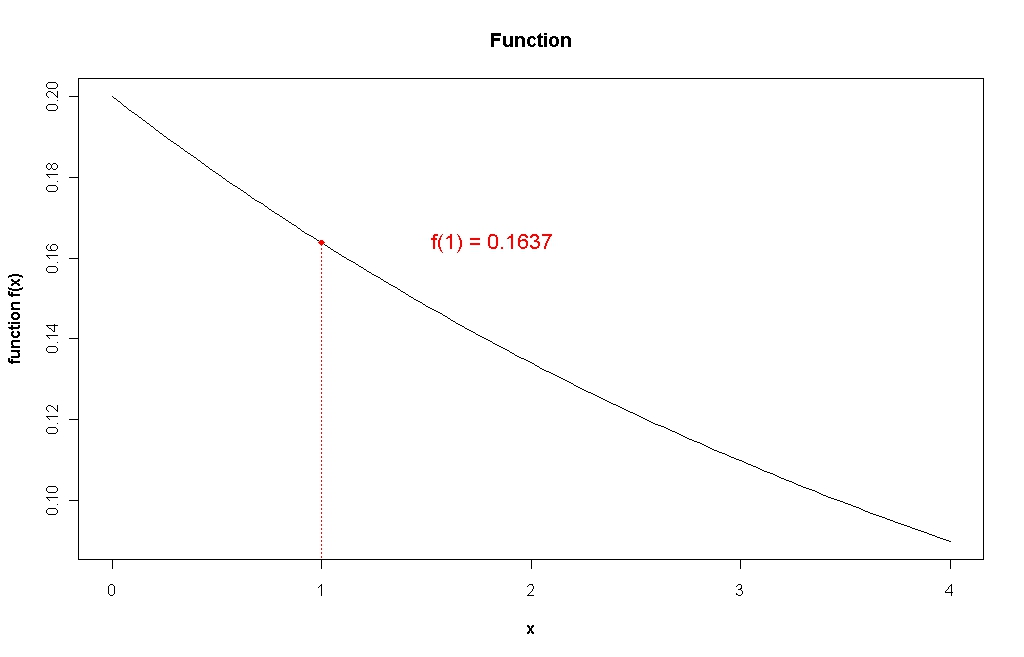
\includegraphics[scale=0.30]{6AFunction}

\end{center}

Some function $f(x)$ evaluated at $x=1$.
\end{frame}
%----------------------------------------------------------------------------------------------------%
\begin{frame}
\frametitle{Definite Integral}

\vspace{-0.5cm}
\begin{center}
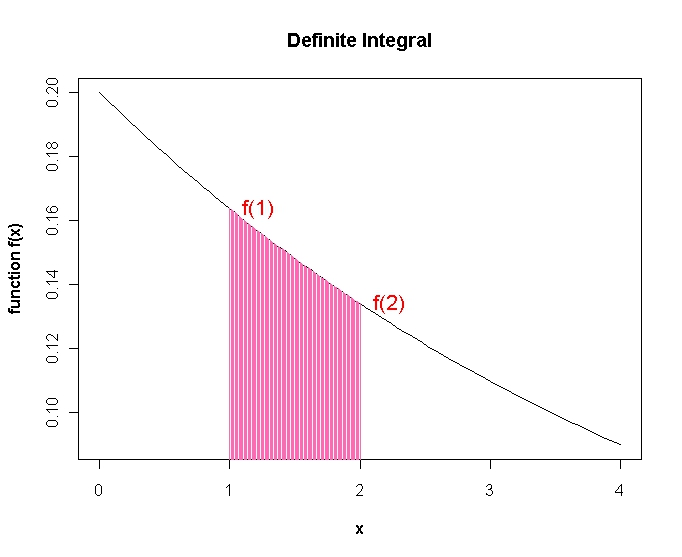
\includegraphics[scale=0.35]{6ADefiniteIntegral}
\end{center}
Definite integral of function is area under curve between X=1 and X=2.
\end{frame}
%----------------------------------------------------------------------------------------------------%
\begin{frame}
\frametitle{Definite Integral}
\begin{itemize}
\item Definite integrals are used to compute the ``area under curves".
\item Definite integrals are defined by a lower and upper limit.
\item The area under the curve between X=1 and  X=2 is depicted in the previous slide.
\item By computing the definite integral, we are able to determine a value for this area.
\item Probability can be represented as an area under a curve.
\end{itemize}
\end{frame}

%----------------------------------------------------------------------------------------------------%
\frame{

\frametitle{Probability Density Function}
\begin{itemize}
\item
In probability theory, a \textbf{\emph{probability density function}} (PDF) (or ``density" for short ) of a continuous random variable is a function that describes the relative likelihood for this random variable to occur at a given point.

\item The PDF for a continuous random variable $X$ is often denoted $f_X(x)$.

\item The probability density function can be integrated to obtain the probability that the random variable takes a value in a given interval.

\item The probability for the random variable to fall within a particular interval is given by the integral of this variable's density over the region.

\item The probability density function is non-negative everywhere, and its integral over the entire space is equal to one.
\end{itemize}
}

\begin{frame}

\frametitle{Density Curves}


\begin{itemize}
\item A plot of the PDF is referred to as a `\textbf{\emph{density curve}}'.
\item A density curve that is always on or above the horizontal axis and has total area underneath equal to one.
\item Area under the curve in a range of values indicates the proportion of values in that range.
\item Density curves come in a variety of shapes, but the normal distribution's bell-shaped densities are the commonly used.
\item Remember the density is only an approximation, but it simplifies analysis and is generally accurate enough for practical use.
\end{itemize}
\end{frame}

%----------------------------------------------------------------------------------------------------%
\frame{
\frametitle{The Cumulative Distribution Function }
Recall:
\begin{itemize}
\item The \textbf{\emph{cumulative distribution function}} (CDF), (or just distribution function), describes the probability that a continuous random variable X with a given probability distribution will be found at a value less than or equal to x.\\

\[ F_X(x) = P(X \leq x) \]

\item Intuitively, it is the ``area so far" function of the probability distribution.
\end{itemize}
}
%----------------------------------------------------------------------------------------------------%
\begin{frame}
\frametitle{Cumulative Distribution Function}

\vspace{-0.5cm}
\begin{center}
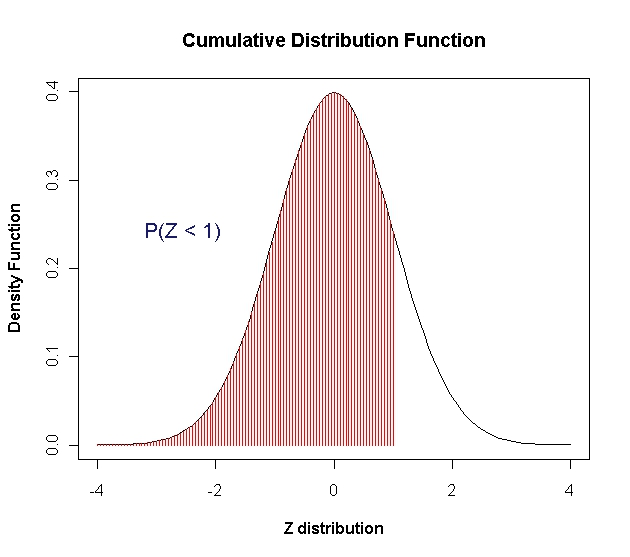
\includegraphics[scale=0.35]{6ACDF}

\end{center}
Cumulative Distribution Function $P(Z \leq 1)$.
\end{frame}


%---------------------------------------------------------------------------%
\frame{
\frametitle{Continuous Uniform Distribution}
A random variable X is called a continuous uniform random variable over the interval $(a,b)$ if it's probability density function is given by
\[ f_{X}(x) = { 1 \over b-a} \hspace{1cm} \mbox{ when } a \leq x \leq b \mbox{     (otherwise } f_X(x) = 0 ) \]
The corresponding cumulative density function is
\[ F_x(x) = { x-a \over b-a} \hspace{1cm} \mbox{ when } a \leq x \leq b\]
}
%----------------------------------------------------------------------------------------------------%
\begin{frame}
\frametitle{The Continuous Uniform Distribution}

\vspace{-0.5cm}

\begin{center}
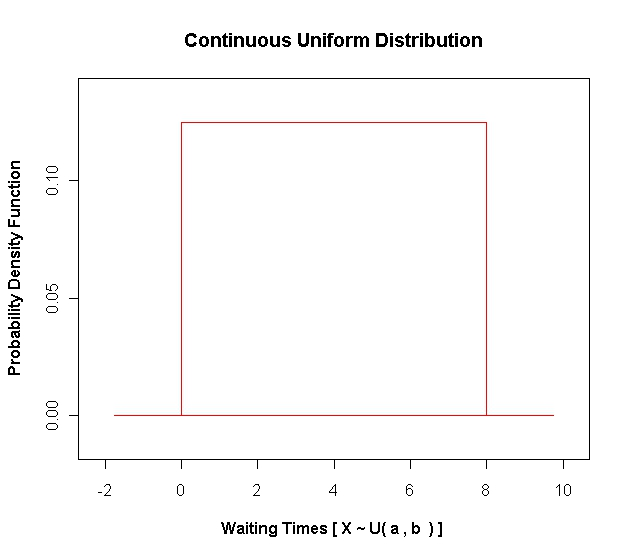
\includegraphics[scale=0.35]{6AUniform}

\end{center}
\end{frame}
%---------------------------------------------------------------------------%
\frame{
\frametitle{Continuous Uniform Distribution}
\begin{itemize}
\item The continuous uniform distribution is very simple to understand and implement, and is commonly used in computer applications (e.g. computer simulation).
\item It is also known as the `Rectangle Distribution' for obvious reasons.
\item We specify the word ``continuous" so as to distinguish it from it's discrete equivalent: the discrete uniform distribution.
\item Remark; the dice distribution is a discrete uniform distribution with lower and upper limits 1 and 6 respectively.
\end{itemize}
}
%-----------------------------------------------------%
\frame{
\frametitle{Uniform Distribution Parameters}


The continuous uniform distribution is characterized by the following parameters

\begin{itemize}
\item The lower limit $a$
\item The upper limit $b$
\item We denote a uniform random variable $X$ as $X \sim U(a,b)$
\end{itemize}

It is not possible to have an outcome that is lower than $a$ or larger than $b$.

\[ P(X < a) = P(X > b) = 0\]
}

%------------------------------------------------------------------------%
\frame{\frametitle{Interval Probability}

\begin{itemize}
\item We wish to compute the probability of an outcome being within a range of values.
\item We shall call this lower bound of this range $L$ and the upper bound $ U$.
\item Necessarily $L$ and $U$ must be possible outcomes.
\item The probability of $X$ being between $L$ and $U$ is denoted $P( L \leq X \leq U )$.

\[
P( L \leq X \leq U ) = { U - L \over b - a}
\]
\item (This equation is based on a definite integral).
\end{itemize}
}

%---------------------------------------------------------------------------------------------------------%
\frame{
\frametitle{Uniform Distribution: Cumulative Distribution}
\begin{itemize}

\item For any value ``c" between the minimum value a and the maximum
value $b$, we can say
\item $P(X \geq c)$ \[P(X \geq c) = {b-c \over b-a}\]
here $b$ is the upper bound while $c$ is the lower bound
\item $P(X \leq c)$ \[P(X \leq c) = {c-a \over b-a}\]
here $c$ is the upper bound while $a$ is the lower bound.
\end{itemize}
}

%-----------------------------------------------------------------------------%
\frame{
\frametitle{Uniform Distribution: Mean and Variance}
\begin{itemize}
\item The mean of the continuous uniform distribution, with parameters $a$ and $b$ is
\[ E(X) = {a+b \over 2}\]
\item The variance is computed as
\[ V(X) = {(b-a)^2 \over 12}\]
\end{itemize}
}
%------------------------------------------------------------------------%
\frame{
\frametitle{Uniform Distribution: Example}

\begin{itemize}
\item Suppose there is a platform in a subway station in a large large city. \item Subway trains arrive \textbf{every three minutes} at this platform. \item What is the shortest possible time a passenger would have to wait for a train?
\item What is the longest possible time a passenger will have to wait?
\end{itemize}

}


%------------------------------------------------------------------------%
\frame{
\frametitle{Uniform Distribution: Example}

\begin{itemize}
 \item What is the shortest possible time a passenger would have to wait for a train?
%\begin{itemize}
\item If the passenger arrives just before the doors close, then the waiting time is zero.
\[ a = 0 \mbox{ minutes } \]
\end{itemize}
}


%------------------------------------------------------------------------%
\frame{
\frametitle{Uniform Distribution: Example}

\begin{itemize}
\item What is the longest possible time a passenger will have to wait?
%\begin{itemize}
\item If the passenger arrives just after the doors close, and missing the train, then he or she will have to wait the full three minutes for the next one.
\[ b = 3 \mbox{ minutes }  = 180 \mbox{ seconds}  \]
\end{itemize}
%\end{itemize}

}

%------------------------------------------------------------------------%
\frame{
\frametitle{Uniform Distribution: Example}

\begin{itemize}
\item What is the longest probability that he will have to wait longer than 2 minutes?
\[ P(X \geq 2)  = {3-2 \over 3-0} = {1/3} = 0.33333   \]
\end{itemize}
%\end{itemize}

}

%----------------------------------------------------------------------------------------------------%
\begin{frame}
\frametitle{The Continuous Uniform Distribution}

\vspace{-0.5cm}

\begin{center}
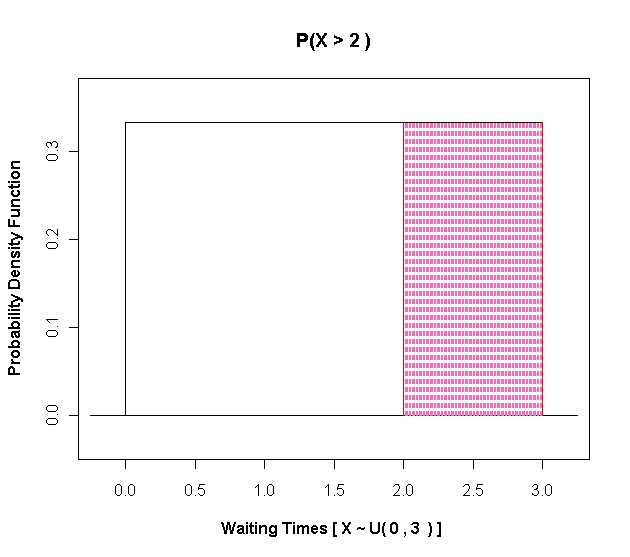
\includegraphics[scale=0.35]{6AUniform4}

\end{center}
\end{frame}
%------------------------------------------------------------------------%
\frame{
\frametitle{Uniform Distribution: Example}

\begin{itemize}
\item What is the longest probability that he will have to wait less than than 45 seconds (i.e. 0.75 minutes)?
\[ P(X \leq 0.75)  = {0.75 - 0 \over 3-0} = {0.75/3} = 0.250  \]
\end{itemize}
%\end{itemize}

}



%----------------------------------------------------------------------------------------------------%
\begin{frame}
\frametitle{The Continuous Uniform Distribution}

\vspace{-0.5cm}

\begin{center}
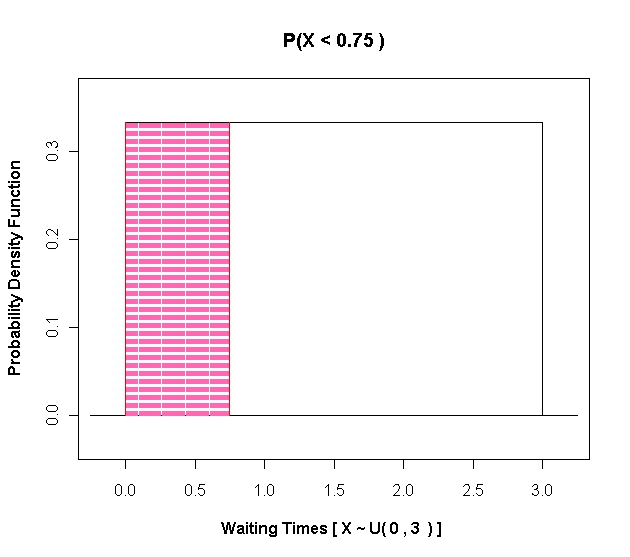
\includegraphics[scale=0.35]{6AUniform3}

\end{center}
\end{frame}
%------------------------------------------------------------------------%
\frame{
\frametitle{Uniform Distribution: Expected Value}

We are told that, for waiting times,  the lower limit $a$ is 0, and the upper limit $b$ is 3 minutes. \\ \bigskip The expected waiting time $\textrm{E}[X]$ is computed as follows
\vspace{0.1cm}
\[
\textrm{E}[X] = {b + a \over 2} =  {3 + 0  \over 2}  = 1.5 \mbox{ minutes }
\]

}
%------------------------------------------------------------------------%
\frame{\frametitle{Uniform Distribution: Variance}

The variance of the continuous uniform distribution, denoted $\textrm{V}[X]$,  is  computed using the following formula
\vspace{0.1cm}
\[
\textrm{V}[X] = {(b - a)^2 \over 12}
\]
\vspace{0.1cm}
For our previous example this is
\[
\textrm{V}[X] = {(3 - 0)^2 \over 12} =  {3^2 \over 12} = {9 \over 12} = 0.75
\]
}


\end{document} 